\documentclass[onesided, 12pt]{scrbook}
\usepackage[utf8]{inputenc}
\usepackage{amsmath}
\usepackage{amsthm} %Para definir ambientes con \newtheorem
\usepackage{amsfonts}
\usepackage{amssymb}
\usepackage{makeidx}
\usepackage{graphicx}
\usepackage{natbib}

\title{Aprendizaje de reglas en el mercado accionario mexicano}
\publishers{Centro de Investigación en Computación, Instituto Politécnico Nacional}
\date{}
\author{David Ricardo Montalván Hernández}

%=========Define los ambientes a utilizar =======%
%Define estilo para dar un salto de línea en el encabezado
%del 'teorema'
\newtheoremstyle{break}
{2ex} %above space
{2ex} %below space
{\itshape} %Body font)
{} %indent amount
{\bfseries} %head font
{:} %post head puncuation
{\newline} %post head space
{}

\theoremstyle{break}
%Definición
\newtheorem{definicion}{Definicion}[chapter]

%Teorema
\newtheorem{teorema}{Teorema}[chapter]

%Algoritmo (Utiliza el ambiente tabbing)

\newtheorem{algoritmo}{Algoritmo}[chapter]
%=================================================%


\begin{document}
\maketitle
\pagenumbering{Roman} %numeración romana con mayúsculas
\renewcommand{\contentsname}{Contenido}
\tableofcontents
\renewcommand{\listfigurename}{Lista de imágenes}
\listoffigures
\renewcommand{\listtablename}{Lista de tablas}
\renewcommand\tablename{Tabla}
\renewcommand{\bibname}{Referencias}
\listoftables

\chapter*{Dedicatoria}
%\chapter*{Agradecimientos}
\chapter*{Resumen}
\chapter*{Abstract}

\pagenumbering{arabic} %Numeración árabe

%=============== INTRODUCCIÓN ================= %
\chapter{Introducción}
\label{capitulo:introduccion}
%Motivación y ¿qué es lo que se busca con este trabajo?
%Objetivo general y objetivos particulares.
%Estructura del trabajo.
El incremento en el poder de cómputo, la digitalización de los mercados financieros (en particular el mercado accionario) y la oportunidad de ganar dinero, son algunos de los factores que han motivado la investigación y desarrollo de algoritmos computacionales enfocados a guiar la toma de decisiones de inversión, en particular, determinar los momentos adecuados para realizar compras o ventas.

A pesar de que la idea básica es comprar barato y vender caro, la incertidumbre y complejidad de los mercados financieros han dado lugar al uso de herramientas computacionales con el fin de guiar la toma de decisiones, concretamente, técnicas relacionadas a la inteligencia artificial han ganado notoriedad.

El objetivo general de este trabajo es proponer una metodología para aprender, de manera automática, un conjunto de reglas \textit{IF..THEN}. Estas reglas se utilizarán para obtener estrategias de inversión cuya ganancia, buscamos, sea superior a la ganancia generada por la estrategia de \textbf{compra y espera} (ver sección \ref{seccion:hipotesis mercado eficiente}).

Una de las contribuciones de este trabajo es el análisis del mercado accionario mexicano, el cual está representado por el instrumento llamado \textbf{NAFTRAC ISHRS} (ver sección \ref{seccion:naftrac}).

Además, la metodología propuesta busca obtener un modelo interpretable, contrastando con la tendencia actual que se caracteriza por el uso de las llamadas \textit{cajas negras}, e.g., redes neuronales (ver capítulo \ref{capitulo:antecedentes}).

Los objetivos particulares de este trabajo son:
\begin{itemize}
\item Selección de atributos.

\item Etiquetado de datos.
\end{itemize}




%=============== Antecedentes ================= %
\chapter{Antecedentes}
\label{capitulo:antecedentes}
\begin{itemize}
\item Explicación de los artículos (en forma cronológica).
\end{itemize}

%=============== Marco teórico ================= %
\chapter{Marco teórico}
\label{capitulo:marco teorico}

\section{Mecánica de un mercado accionario.}
\label{seccion:mecanica del mercado}

\section{Hipótesis del mercado eficiente.}
\label{seccion:hipotesis mercado eficiente}

\section{Costos de transacción}
\label{seccion:costos de transaccion}

\section{NAFTRAC.}
\label{seccion:naftrac}

\section{SPDR S\&P 500}
\label{seccion:sp500}

\section{Análisis técnico}
\label{seccion:analisisTecnico}

\section{Supuestos del trabajo}
\label{seccion:supuestos}


%=============== AQ y CN2 ================= %
\section{Algoritmos AQ y CN2}
\label{seccion:algoritmos aq cn2}

\subsection{Algoritmo AQ}
\label{subseccion:algoritmo aq}

\subsection{Algoritmo CN2}
\label{subseccion:algoritmo cn2}

%=============== Solución propuesta ================= %
\chapter{Solución propuesta}
\label{capitulo:solucion propuesta}

\section{Separación de datos}
\label{seccion:separacion de datos}
En este trabajo se utilizan precios diarios\footnote{Obtenidos de Yahoo Finance. https://finance.yahoo.com} de los instrumentos NAFTRAC y SPDR S\&P 500 (ver secciones \ref{seccion:naftrac} y \ref{seccion:sp500}).

Para el NAFTRAC, la información inicia el día 15 de febrero de 2013 y termina el 21 de enero de 2019. Para el SPDR S\&P 500 el periodo de tiempo abarcado es del 2 de enero de 2008 hasta  el 3 de marzo de 2019.

La tabla \ref{tabla:Ejemplo datos diarios NAFTRAC} muestra la estructura de los datos para el NAFTRAC. Es importante señalar que los datos no incluyen días festivos y fines de semana.

\begin{table}[h]
\centering
\begin{tabular}{cccccccc}
\hline
\textbf{Fecha} & \textbf{Apertura} & \textbf{Máximo} & \textbf{Mínimo} & \textbf{Cierre} & \textbf{Cierre ajustado} & \textbf{Volumen} \\
\hline
2013/02/15 & 44.09 & 44.24 & 43.86 & 44.18 & 41.61 & 77,614,608\\
2013/02/18 & 44.38 & 44.38 & 44.04 & 44.16 & 41.60 & 6,457,428\\
2013/02/19 & 44.34 & 44.77 & 44.29 & 44.63 & 42.05 & 68,042,072\\
\vdots & \vdots & \vdots & \vdots & \vdots & \vdots & \vdots \\
\hline
\end{tabular}
\caption{\label{tabla:Ejemplo datos diarios NAFTRAC} Datos diarios NAFTRAC}
\end{table}

Para crear nuestros conjuntos de entrenamiento y prueba, los datos se dividen utilizando una ventana deslizante de 90 días. Este criterio está fundamentado en el hecho de que, tanto en México como en Estados Unidos, las empresas con acciones listadas en alguna bolsa de valores, están obligadas a reportar los resultados de sus operaciones de manera trimestral, así pues, buscamos capturar la reacción de los inversionistas ante la publicación de dicha información.

La tabla \ref{tabla:data split SP500} muestra la separación de los datos del SPDR S\&P 500.
\begin{table}[h]
\centering
\begin{tabular}{cc}
\hline
\textbf{Entrenamiento} & \textbf{Prueba} \\
\hline
2008/01/02 - 2008/05/09 & 2008/05/12 - 2008/09/17 \\
2008/05/12 - 2008/09/17 & 2008/09/18 - 2009/01/27 \\
2008/09/18 - 2009/01/27 & 2009/01/28 - 2009/06/05 \\
\vdots & \vdots \\
\hline
\end{tabular}
\caption{\label{tabla:data split SP500} Separación de datos}
\end{table}

Utilizando esta metodología para la separación de datos, se obtienen 15 conjuntos de entrenamiento y 15 conjuntos de prueba con la información del NAFTRAC, por otra parte, para los datos del SPDR S\&P 500 se obtienen 30 conjuntos de entrenamiento y 30 conjuntos de prueba.

\section{Proceso de etiquetado}
\label{seccion:proceso etiquetado}
Ya que nuestros datos de entrenamiento no están etiquetados, utilizamos un algoritmo evolutivo para obtener un conjunto de etiquetas que nos permita entrenar cada modelo.

Este algoritmo evolutivo pertenece a la clase de algoritmos para la estimación de distribución (EDA por sus siglas en inglés \cite{simon2013evolutionary}). Cada individuo en la población representa una estrategia de inversión para un periodo de prueba dado. Esta estrategia está representada a través de un vector $\mathbf{x} = (x_1, x_2, \ldots, x_t)$ cuya componente $x_i$ representan la acción a tomar en el día $i$, $x_i \in \{-1,0,1\}$, en donde $-1$ representa una señal de venta, $0$ una señal de espera y $1$ una señal de compra. La función de aptitud utilizada fue el exceso de ganancia sobre la estrategia buy-and-hold.

Vemos entonces que,  la idea detrás del etiquetado se basa en encontrar las combinaciones de compras y ventas que nos generen la mayor ganancia una vez conocida toda la historia del periodo de entrenamiento.

\begin{figure}[h]
\centering
\scalebox{0.85}{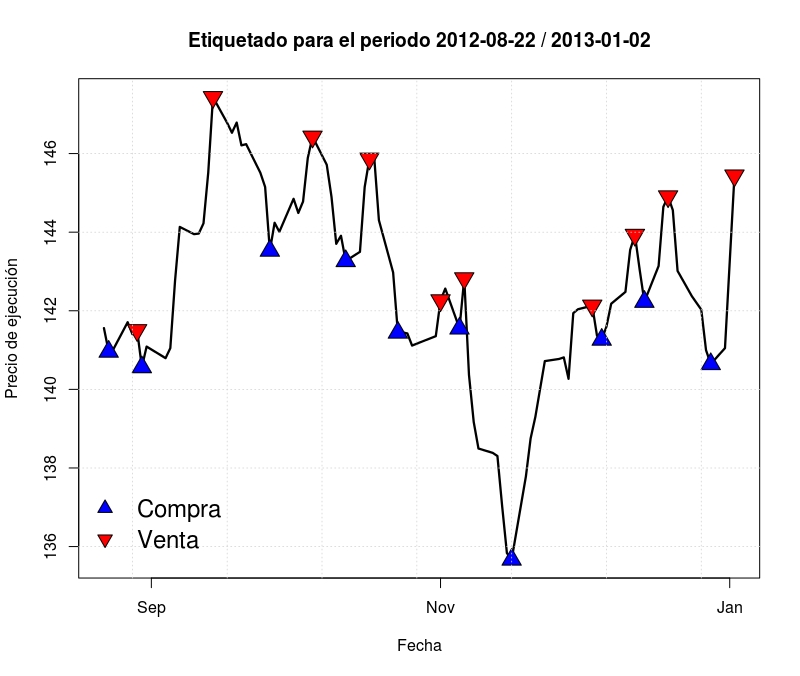
\includegraphics[width=1\linewidth]{imagenes/etiquetado.jpeg}}
\caption{\label{imagen:etiquetado} Proceso de etiquetado}
\end{figure}

\section{Atributos utilizados}
\label{seccion:atributos}
Los atributos utilizados en cada uno de los experimentos, son un conjunto de indicadores técnicos financieros (ver sección \ref{seccion:analisisTecnico}). Utilizamos estos indicadores ya que en ellos se refleja el conocimiento de los expertos, así como patrones que han demostrado ser útiles en la práctica.

Los indicadores utilizados son:
\begin{itemize}
\item Oscilador Aroon con una ventana de tiempo de 25 días para cada cada indicador Aroon.

\item RSI con una ventana de tiempo de 14 días.

\item MFI con una ventana de tiempo de 14 días.

\item Williams \%R con una ventana de tiempo de 14 días.

\item CCI con una ventana de tiempo de 20 días y un factor $C=0.015$.
\end{itemize}


\section{Aprendizaje incremental}
\label{seccion:aprendizaje incremental}

%=============== Resultados ================= %
\chapter{Resultados experimentales}
\label{capitulo:resultados experimentales}

%=============== Conclusión ================= %
\chapter{Conclusiones y trabajo futuro}
\label{capitulo:conclusiones}

\section{Conclusiones}
\label{seccion:conclusiones}

\section{Trabajo futuro}
\label{seccion:trabajo futuro}


\bibliography{references}
\bibliographystyle{plain}
%\bibliographystyle{elsarticle-harv.bst}






\end{document}